%==========================================================================
%Template File for Monthly Lectual Meeting
%2006/05/22 (kkobayashi@mikilab.doshisha.ac.jp)
%==========================================================================
\documentclass[a4j,9pt,twocolumn]{jsarticle}
\usepackage{mlm2.0}
\usepackage{epsf}
\pagestyle{plain}
\usepackage{url}
\usepackage{subfigure}
\setcounter{page}{1}
\usepackage{geometry}
\geometry{left=25mm,right=25mm,top=20mm,bottom=30mm}
%\usepackage[dvips]{graphicx}

\begin{document}
\twocolumn[
%---------------------------------------------------------------------------        % ヘッダ    書式:\beginheader{回}{年}{月}
%---------------------------------------------------------------------------
\beginheader{171}{2016}{04}
%---------------------------------------------------------------------------
% 発表題目    書式:\title{日本語}{英語} 「\\」で改行できます
%---------------------------------------------------------------------------
\title%
{git}%
%{更なる大容量化を目指して 進化しつづける次世代光メディア}

%---------------------------------------------------------------------------
% 著者名      書式:\author{日本語著者名}{英語著者名}
%---------------------------------------------------------------------------
\author{山下 俊樹,外村 篤紀\\Toshiki YAMASHITA,Atsuki TONOMURA}

%---------------------------------------------------------------------------
\endheader
%\begin{abstract}
%---------------------------------------------------------------------------
%Recently, a DVD attracts attention along with the image and the digitization of the sound. The standards of these DVD are complicated. So, in this paper, the standards of the DVD are summarized and the DVD of the next generation is refered. 
%---------------------------------------------------------------------------
%\end{abstract}
]

%---------------------------------------------------------------------------
% 本文
%---------------------------------------------------------------------------

\section{はじめに}
近年,ソフトウェアの大規模化にともない,プログラムの開発頻度は増加傾向にある.システムによる管理を行わず,開発に使用するファイルを編集した場合を考える.この場合,ファイルを以前の状態に復元したい時に,復元したい状態のファイルが発見しづらいなどの不具合がある.そこで,コンピュータ上で作成または編集したファイルの変更履歴を管理するバージョン管理システムは,より重要となっている.本稿では,バージョン管理システムの1つであるgit,および関連サービスのGitHubについて述べる.

\section{git}
\subsection{概要}
gitはバージョン管理システムの1つであり,CUIで動作する.バージョン管理システムは,管理しているファイルを以前の状態に戻す機能や,複数人で1つのファイルを編集するときに発生してしまう競合を解消する機能を持つ.これらの機能を用いることで,開発中にバグが発生した場合,ファイルをバグが発生する以前の状態に復元できるなどの利点がある\cite{pop}.

\subsection{構成}
gitで管理されるファイルやフォルダの変更内容は,リポジトリと呼ばれるデータベースに蓄積される.分散型バージョン管理システムにおけるリポジトリは2種類に大別できる.gitの構成を\fgref{git}に示す.

\begin{figure}[h]
\centering
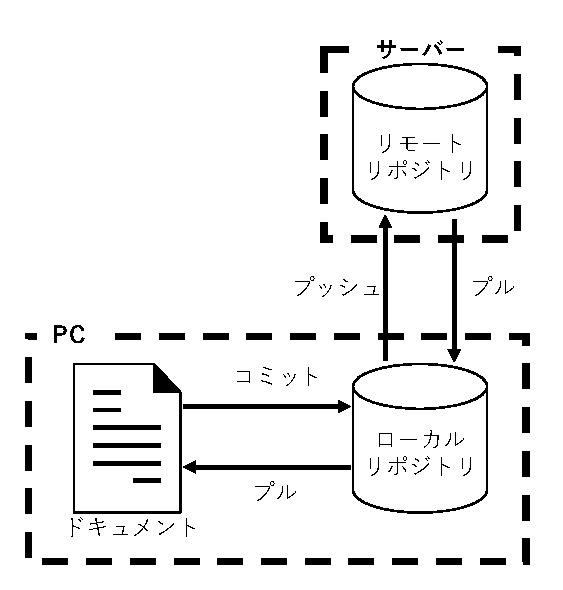
\includegraphics[width=80mm]{img/git.eps}
\caption{gitの構成}
\label{git}
\end{figure}

ローカルリポジトリは,個人のPC内に配置され,個人で利用する.ファイルやフォルダの変更をローカルリポジトリに記録する操作をコミットと呼ぶ.コミットやプッシュを行うことで作業成果を記録する.ローカルリポジトリによって,ネットワークに接続されていない環境でもコミットを行うことができる.

リモートリポジトリは,サーバ上に配置され,複数ユーザで利用する.プルを行うことでリモートリポジトリから他者の作業成果をダウンロードしてローカルリポジトリに統合する.例えば,バグ修正のために個人のローカルリポジトリに適量のコミットを行い,修正を完了したとする.その後,修正が完了したソフトウェアをリモートリポジトリにプッシュし,他者に公開する方法が可能である.

\subsection{バージョン管理}
gitは,履歴を管理するファイルを全て蓄積しており,必要なファイルを適切に取り出すことによりバージョン管理を実現している.バージョン管理の例を\fgref{tree}に示す.

\begin{figure}[h]
\centering
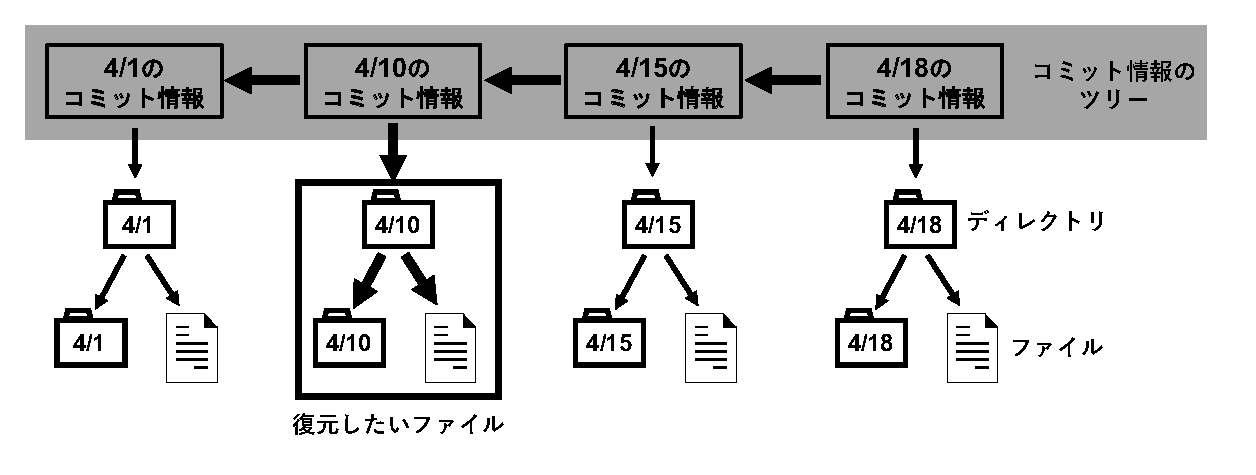
\includegraphics[width=90mm]{img/tree.eps}
\caption{バージョン管理の例}
\label{tree}
\end{figure}

コミットを行うと,コミット情報,および履歴を管理しているファイルがリポジトリに保存される.コミット情報は以下の2つで構成される.

\begin{itemize}
\item コミットしたファイルの保存場所
\item 前回のコミット情報の保存場所
\end{itemize}

前回のコミット情報の保存場所を辿ることで,復元したいファイルやフォルダにアクセスできる.

\subsection{ブランチ}
gitの特徴の1つであるブランチは,蓄積されたコミットの時系列を指す.すなわち,複数回のコミットを作成順に並べた連なりをブランチと呼ぶ.また,ブランチを分岐する操作もブランチと呼ぶ.分岐したブランチ同士は互いに独立しており,異なる内容の更新を同時に行える.ブランチ同士の結合はマージと呼ぶ.ブランチを利用した例を\fgref{branch_ex}に示す.

\begin{figure}[h]
\centering
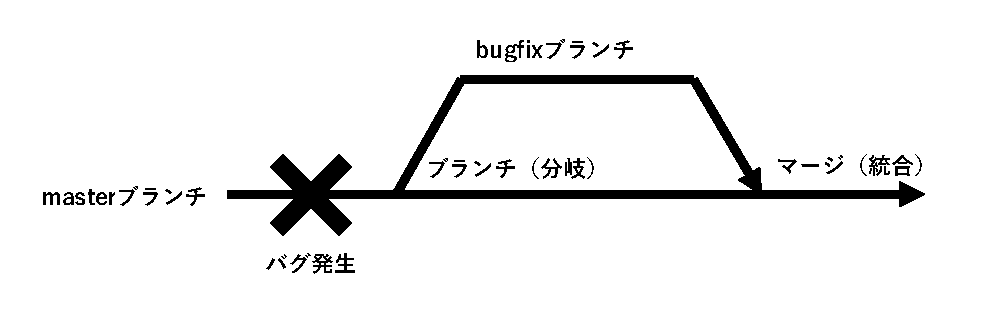
\includegraphics[width=80mm]{img/branch.eps}
\caption{ブランチの例}
\label{branch_ex}
\end{figure}

ブランチを用いることで,様々な開発やバグ修正などを並行して行うことができる.\fgref{branch_ex}において既に運用されているソフトウェアの管理を行っているブランチをmasterブランチとし,そのソフトウェアのバグを修正するために用意したブランチをbugfixブランチとする.この場合,二つのブランチは独立しているため,masterブランチに影響を与えることなくbugfixブランチでバグ修正を行うことができる.すなわち,ブランチを用いない場合は,バグ修正が完了するまでソフトウェアの運用を停止しなければならない.それに対し,ブランチを用いれば,ソフトウェアの運用を止めることなく,平行してバグ修正を行うことができる.バグ修正が完了した後にマージを行った時点でバグが修正される.さらに,ブランチの本数を増やせば,リリースしたソフトウェアを運用しながら新機能の追加を行い,加えてバグ修正も同時に行うといった運用が可能である.

gitのブランチは,他のバージョン管理システムに比べて優れている.他のシステムでは,マージの際にどのファイルをどのようにマージするか明示的に入力する必要があるが,gitは自動的に行うことができる.管理するファイルが多い場合,手動でマージの指示を入力するには労力を要する.しかし,gitのように自動的にマージを行えれば,労力を節約できる.

\section{GitHub}
\subsection{概要}
GitHubとは,gitを利用したSNSである.現在,Githubは最も人気のあるgitサービス提供サイトであり,そのユーザ数は1000万人を超えている\cite{github}.GitHubの特徴の1つは,分かりやすいGUIである.また,リモートリポジトリを利用するには個人でサーバを用意する必要がある.しかし,GitHubのユーザはリモートリポジトリを無料で提供するため,他のユーザと協力してソースコードを管理できるサービスとして広まった.他のユーザと協力するための機能として,コードレビュー,およびコメント機能がある.コードレビューとは,ソースコードに含まれる誤りを検出,修正することを目的として行われるソースコードの査読を指す.これらの機能を用いることで,ユーザのソースコードの評価を他のユーザが行う.その結果,ユーザによる修正が行われ,ソースコードのバグの解消や可読性の向上などの利点を生む.

\subsection{GitHubにおけるブランチの活用例}
gitのブランチの分岐は,GitHubではフォークと呼ばれる.GitHubのユーザは他のユーザのリポジトリからフォークしたアプリケーションを開発することができる.フォークに1つのタスクを割り当てることでチケット駆動開発を行うことができる.

次に,チケットについて述べる.GitHub内ではIssuesと呼ばれているが,本稿ではチケットと同義とする.チケットとは,作業をタスクに分割し,タスク1つ1つに対して割り振られるものである.開発者は発行されたチケットを取り,チケットに記されたタスク(バグ修正や機能追加など)をこなす.タスクが完了するとコミットを行い,チケットを消去(クローズ)する.

タスクをチケットで管理することにより,作業の全容が把握しやすいことや,チームでの開発においてタスクの分配が行いやすくなる利点がある.また,チケットを用いて行うチケット駆動開発は,アジャイル開発とも親和性が高いため,注目を集めている.アジャイル開発とは,開発対象を多数の小さな機能に分割し,短い期間(1週間から4週間)で1つの機能を開発する工程を反復し,開発を行う手法である.アジャイル開発における小さな機能にチケットを割り当てることで,チケット駆動開発との統合を実現する.チケット駆動開発を行う際には,オンラインプロジェクト管理ソフトウェアであるRedmineを併用する場合が多い.

一方,欠点として,GitHubで作成したリモートリポジトリは全て公開されるため,ソースコードを公開できないWebデザインや個人情報を扱う開発などのソースコード管理には不具合が発生する.また,GitHubはインターネット上のサーバを用いるため,サーバ障害などが発生した場合にサービスが使用不能になる.実際に,2016年1月28日にサービス障害が発生し,多くのユーザや企業が被害を被った\cite{news}.

\subsection{BitBucketとの比較}
GitHubに競合するサービスとして,BitBucketが挙げられる. Githubに対して,非公開のリモートリポジトリを作成できる,およびgit以外の分散型バージョン管理システムであるMercurialを使用できる利点がある.どちらのサービスもソーシャルコーディングの普及に貢献しているが,現時点でのユーザ数はGitHubが圧倒的に多い.これは,GitHubに対応する周辺サービスが多いことや,GUIが使いやすいことなどによる.

\section{今後の展望}
今日,ソフトウェアのリリース速度は増加の一途を辿っている.それにともない,開発の効率化,高速化が重要視されている.そのため,gitのようなバージョン管理ソフトウェアは更に普及すると考えられる.gitが普及すると,開発が複数の開発者や企業の間で効率よく分配されると思われる.

\small
\begin{thebibliography}{99}
\bibitem{pop}
岡本隆史:Gitに潜む光と闇,入手先,(http://gihyo.jp/dev/column/01/prog/2012/git)

\bibitem{mecha}
koseki2:Git の仕組み (1),入手先(http://koseki.\\hatenablog.com/entry/2014/04/22/inside-git-1)

\bibitem{github}
Ken Nishimura,市民生活をオープンデータ活用で改善する政府や地域行政の事例 [GitHub Universe],(http://thebridge.jp/2015/10/github-universe-session-changing-lives-with-open-data).

\bibitem{news}
Yukari Mitsuhashi,GitHub、1月末のダウンの原因はデータセンターでの停電と説明,(http://www.itmedia.co.jp/news/articles/1602/\\01/news070.html).
\end{thebibliography}
\end{document}